\documentclass{article}
\usepackage[utf8]{inputenc}
\usepackage[spanish]{babel} % Para poder escribir tildes y ñ en español
\usepackage{graphicx}
\usepackage{float}
%agregar notas al pdf
\usepackage{todonotes}
\presetkeys{todonotes}{inline}{} 

%caracteristicas de páginas
\pdfpagewidth 8.5in
\pdfpageheight 11in
\setlength\oddsidemargin{-0,21in}
\setlength\evensidemargin{-0,21in}
\setlength\topmargin{-2cm}
\setlength\textwidth{7in}
\setlength\textheight{23.7cm}
\setlength\parskip{0.1in}
\usepackage{multicol}
\setlength{\columnsep}{1cm}


\title{tp-aprendizaje}
\author{seba vita}
\date{September 2016}


\begin{document}
\thispagestyle{empty}
\begin{center}

\Huge{ \bf{UNIVERSIDAD DE BUENOS AIRES}}
\\
\LARGE{\bf{Facultad de Ciencias Exactas y Naturales}}
\\
\textbf{Departamento de Computaci\'on}
\\
\textbf{Aprendizaje Automático}
\vspace{2.0\baselineskip}
\end{center}


\begin{figure}[H] %[h] Aqui [b] para button [t] para top
\begin{center}
\includegraphics[width=100pt]{uba.jpg}
\end{center}
\end{figure}
\begin{center}
\vspace*{0.5cm}

\huge{\bf TRABAJO PR\'ACTICO N\'UMERO 1}\\
\huge{Detección de Spam}
\vspace*{1.6cm}

\end{center}

\LARGE {\textbf{Alumnos:}}\\
\Large{\textsl{Corbat, Agustin} \hspace{1.59cm}$|$ agustin.corbat@gmail.com}\\
\Large{\textsl{Sanchez Cano, Gonzalo} $|$ gonzalo.sanchezcano@gmail.com}\\
\Large{\textsl{Vita, Sebasti\'an} \hspace{1.79cm}$|$ sebastian\_vita@yahoo.com.ar}
\vspace{0.6cm}



\vspace*{1cm}
 
\newpage


\section{Introducción}

El objetivo del presente trabajo es desarrollar y entrenar un modelo basado en aprendizaje automático capaz de separar correo electrónico \textit{spam} de correo electrónico \textit{ham}. Para ello se utilizó un conjunto de correos previamente clasificados como datos de entrenamiento de los distintos modelos a probarse. Dicho conjunto fue seccionado inicialmente de forma aleatoria en un conjunto que consistía en el 80$\%$ de los datos para entrenamiento, y dos secciones de 10$\%$ cada una utilizadas para evaluar el modelo entrenado, disminuyendo así el riesgo de sobreajuste a los datos utilizados para entrenamiento.

En primer lugar, fue necesario extraer diversos atributos de los correos que podrían ser o no utilizados posteriormente por el modelo como parámetros para clasificarlos. A continuación, se eligieron y estudiaron cinco clasificadores distintos, a saber \textbf{Naive Bayes} (\textbf{NB}), \textbf{Decision Tree} (\textbf{DT}), \textbf{k-Nearest Neighbours} (\textbf{kNN}), \textbf{Support Vector Machines} (\textbf{SVM}) y \textbf{Random Forests} (\textbf{RF}), para evaluar su eficiencia a la hora de predecir si un correo se trata de \textit{spam} o no.

Una vez completada la primer evaluación, se procedió a estudiar la posible mejora introducida al modelo al utilizar alguna de dos posibles reducciones de dimensionalidad, \textit{Principal Component Analysis} (\textbf{PCA}) o \textit{Latent Semantic Analysis} (\textbf{LSA}). Dichas mejorías fueron evaluadas aplicando los dos mejores clasificadores que surgieron del estudio anterior.

Habiendo hallado el mejor clasificador y la mejor combinación de clasificador con su método de reducción de dimensionalidad, se evaluó como respondían ambos a la hora de predecir la clasificación de una de las secciones de datos correspondiente a la evaluación. En caso de que este resultado sea desfavorable, sería necesario rever los atributos extraídos así como los clasificadores y métodos de reducción de dimensionalidad elegidos. Por otro lado, si los resultados son favorables, entonces el último conjunto de datos servirá como cierre de la evaluación del clasificador elegido.

\section{Extracción de atributos}

Como se mencionó previamente, el primer paso a la hora de entrenar un modelo es seleccionar y extraer de forma creativa y adecuada los atributos de los correos que puedan llegar a resultar útiles para clasificarlos en las categorías propuestas.

En primer lugar, se utilizaron como atributos posibles la longitud del correo completo, así como la cantidad de espacios que contiene. Dichos atributos fueron propuestos como ejemplo y se mantuvieron durante la extracción. Por otro lado, se calcularon la cantidad de caractéres especiales dentro del cuerpo del correo. Además, esto esta altamente correlacionado con la posibilidad de que el mismo contenga o no código html que, a su vez, se relaciona con una alta probabilidad de que se trate de un correo \textit{spam}.

A continuación, se apreció que la presencia o ausencia de ciertos campos de la cabecera de los distintos correos podían dar indicios de si se trataba de \textit{spam} o no. Luego se procedió a evaluar cuales eran todas las posibilidades y se extrajo para cada correo la presencia o ausencia de dichos campos.

Por otro lado, resulta interesante estudiar qué sucede cuando un correo corresponde a una respuesta a otro correo. Pudo apreciarse que los correos que eran respuestas a otro correo (poseen alguna variante de 're:' en el asunto) corresponden a \textit{ham} con una frecuencia del orden de mil veces más alta que para \textit{spam}.

Finalmente, se realizó un recuento de correos que presentan alguna palabra en particular en el asunto. Se tomaron las 300 palabras más frecuentemente encontradas en el asunto de correos de \textit{spam}, y se descartaron las que pertenecían a las 3000 palabras más comunes de \textit{ham}, y viceversa. De esta forma, se pretendía seleccionar de forma diferencial las palabras comunes a una categoría de correos y no a la otra. Se computó la presencia o ausencia de estas palabras en el asunto como atributo de los correos.

\section{Clasificadores}

Habiendo finalizado la etapa de extracción de atributos, en la cual se obtuvieron 1105 atributos distintos, se prosiguió con el entrenamiento y clasificación de los correos con los modelos planteados y presentados a continuación. En particular, se plantearon los clasifacores de \textbf{Naive Bayes} (\textbf{NB}), \textbf{Decision Tree} (\textbf{DT}), \textbf{k-Nearest Neighbours} (\textbf{kNN}), \textbf{Support Vector Machines} (\textbf{SVM}) y \textbf{Random Forests} (\textbf{RF}).

\subsection{Naive Bayes}

Desde el punto de vista de la probabilidad, nuestro objetivo puede cumplirse si conocemos la probabilidad de que un correo pertenezca a cierta categoría dado los atributos que posee. En particular, podemos utilizar el teorema de Bayes para expresar dicha probabilidad en función de la probabilidad de que posea ciertos atributos dada la categoría a la que pertenece. Una vez hecho esto, podríamos usar una hipótesis ingenua al considerar independientes sus variables para separar el sistema y facilitar el cálculo de la probabilidad buscada. 

Considerando que la gran mayoría de los atributos extraídos correspondía a valores binarios, y teniendo en cuenta que en caso de no ser binarios estos pueden binarizarse, se procedió a utilizar el clasificador de Bernouilli de Naive Bayes. Se presenta a continuación una tabla de los resultados hallados al realizar 10 cross validation con dicho clasificador. El tiempo de ejecución de dicho entrenamiento fue de 21 segundos.


%Considerando que nuestro objetivo es predecir si un correo pertenece a cierta categoría dado que posee ciertos atributos, podemos analizarrlo desde el punto de vista probabilístico calculando la probabilidad de que pertenezca a dicha categoría 

\begin{center}
  \begin{tabular}{| l | c | c |}
    \hline
      & Porcentaje (\%) & Desvío estándar  \\ \hline
    Accuracy & 0.93445834 & 0.00169017242919 \\ \hline
    F1 & 0.93757367 & 0.00153662419091 \\ \hline
    Precision & 0.89505954 & 0.00259349457728 \\ \hline
    Recall & 0.98433333 & 0.0013505572243 \\
    \hline
  \end{tabular}
\end{center}

\subsection{K vecinos más cercanos (KNN)}

Otro modelo de clasificador evaluado es el de k-vecinos más cercanos. En este caso, las instancias son ubicadas según sus atributos y se utiliza la distancia euclidiana para medir la separación entre las mismas. 

El hiperparámetro que variamos a la hora de experimentar fue la cantidad de vecinos que se tenían en cuenta en la votación de si una instancia pertenecía a una u otra categoría. Para esto, decidimos probar con cantidades impares de vecinos ya que, en caso de empate, siempre hubiese alguna instancia capaz de desempatar.

\begin{figure}[H] %[h] Aqui [b] para button [t] para top
\begin{center}
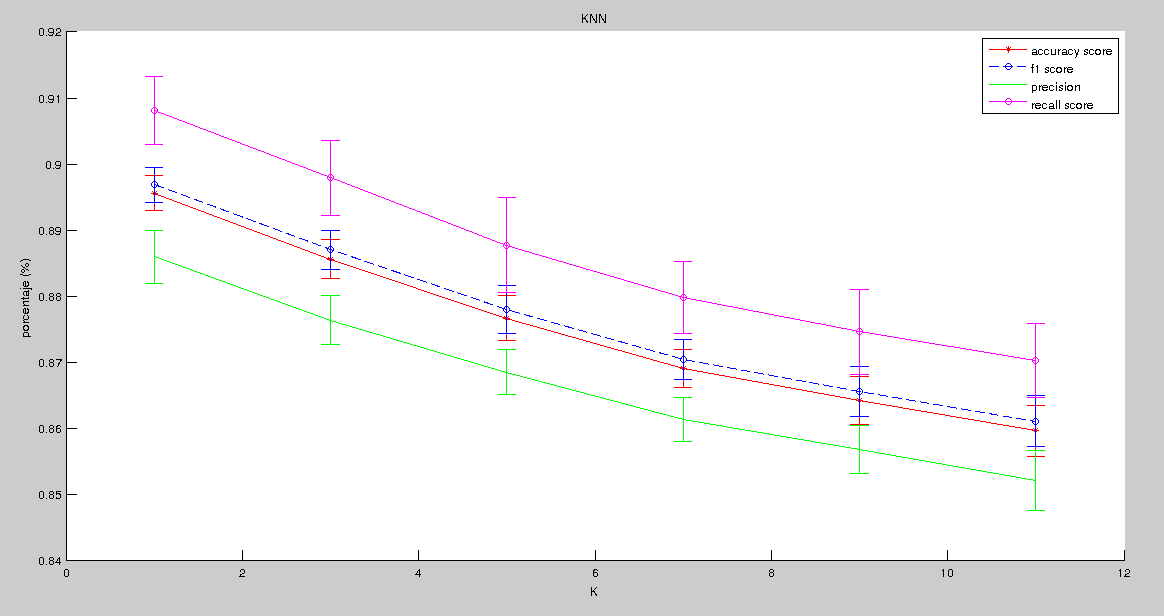
\includegraphics[width=500pt]{knnScores.png}
\caption{KNN variando la cantidad de vecinos más cercanos. Se utilizó el desvío estándar como estimación de la variación en el parámetro evaluado.}
\label{knn}
\end{center}
\end{figure}

Como se muestra en la figura \ref{knn}, cuantos menos vecinos se consideren en la votación, mejor será el resultado. Esto puede explicarse mediante la consideración del ruido que surge de considerar varios vecinos para la votación. En estos casos, los tiempos de entrenamiento variarion en el intervalo de $45\pm5$ segundos.

\subsection{Support vector machines (SVM)}

Para casos donde la cantidad de atributos es elevada y nos define un espacio de alta dimensionalidad, se puede utilizar un clasificador basado en SVM. Estos se utilizan distintos kernels para transformar el espacio de atributos a uno con una dimensión mayor que permita trazar un hiperplano para separar las categorías en cuestión.

\begin{center}
  \begin{tabular}{| l | c | c |}
    \hline
      & Porcentaje (\%) & Desvio estandar  \\ \hline
    Accuracy & 0.89434723 & 0.00285722950847 \\ \hline
    F1 & 0.89071274 & 0.00302317414523 \\ \hline
    Precision & 0.92243407 & 0.00330961589223 \\ \hline
    Recall & 0.86111112 & 0.00409192844458 \\
    \hline
  \end{tabular}
\end{center}

Como se muestra en la tabla, este método no resulta ser de los más eficientes. Una explicación posible es que este clasificador es bueno cuando la cantidad de atributos es mayor a la cantidad de instancias, hecho que se da a la inversa en nuestro caso. El tiempo de entrenamiento de este clasificador fue de alrededor de 2 horas y media.
% 9161 segundos -> 152 min -> 2 horas y media

\subsection{Decision Tree}

En el caso de árboles de decisión, la predicción de la categoría a la cual pertenece una instancia se consigue a partir de decisiones simples inferidas de los atributos de los datos. En este caso, se estudia que atributos separan mejor en categorías a las distintas instancias. Aunque estos árboles podrían tener tantas bifurcaciones como atributos, muchas veces se los truncan a distintas alturas para evitar el sobreajuste.

\begin{figure}[H] %[h] Aqui [b] para button [t] para top
\begin{center}
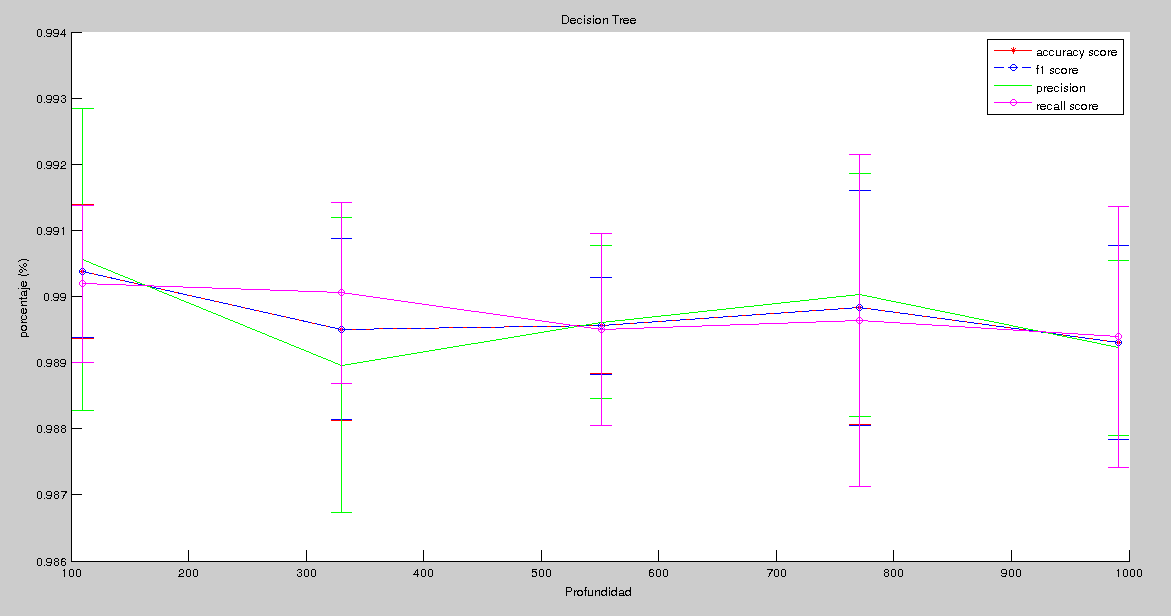
\includegraphics[width=500pt]{decisionTreeScores.png}
\caption{Decision Tree con la altura del árbol variable y la cantidad de atributos $=$ $\sqrt{cantidad\ original\ de\ atributos}$}
\label{DecisionTree}
\end{center}
\end{figure}

En la figura \ref{DecisionTree} se muestran los resultados de haber utilizado árboles de distinta profundidad para entrenar el clasificador. Puede apreciarse fácilmente que los resultados no pueden diferenciarse unos de otros estadísticamente ya que todos caen dentro del intervalo comprendido entre el promedio $\pm$ un desvío estándar. Cabe destacar que los tiempos de entrenamiento de este clasificador fue de aproximadamente 1.7 segundos para todos los casos.

\subsection{Random Forest}

Habiendo introducido al árbol de decisión como un posible clasificador, debemos tener en cuenta que podríamos generar varios árboles de decisión, entrenándolos con distintos subconjuntos de datos. Utilizar la combinación de la información provista por varios árboles para predecir la categoría de una única instancia nos permitirá mejorar la predicción así como también reducir la varianza de su eficiencia. En este caso, no solo podremos variar la profundidad de los árboles generados, sino que también podremos estudiar la cantidad de atributos a considerar y la cantidad de árboles a entrenar.

\begin{figure}[H] %[h] Aqui [b] para button [t] para top
\begin{center}
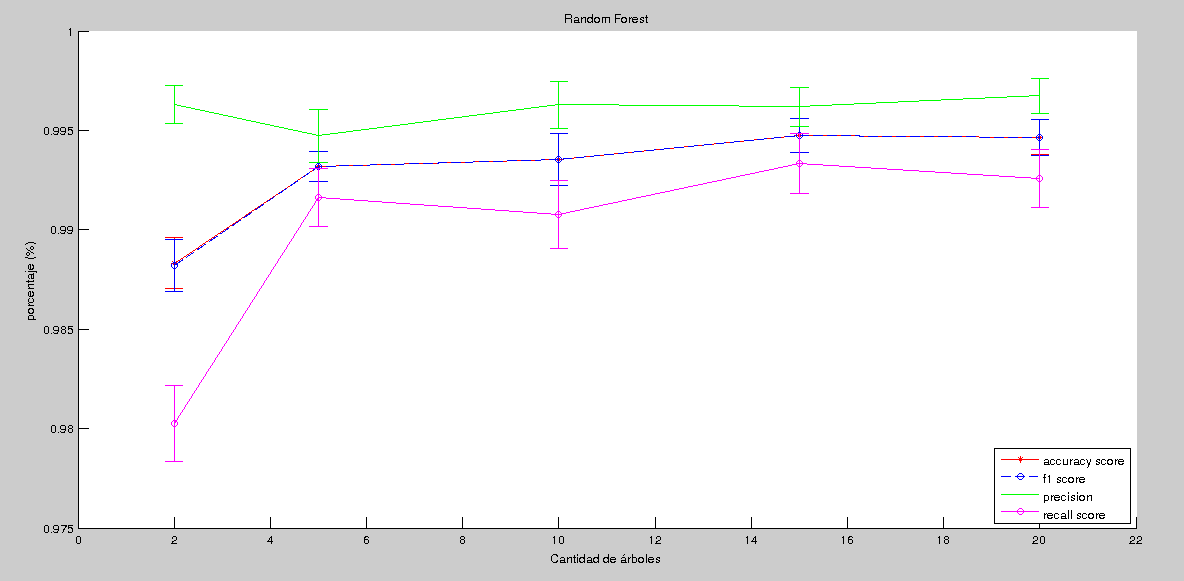
\includegraphics[width=500pt]{randomForestScoreArboles.png}
\caption{Random Forest con la cantidad de árboles variable, cantidad de features $=$ $\sqrt{cantidad\ original\ de\ features}$ y sin restricciones de altura}
\label{randomForestArboles}
\end{center}
\end{figure}

\begin{figure}[H] %[h] Aqui [b] para button [t] para top
\begin{center}
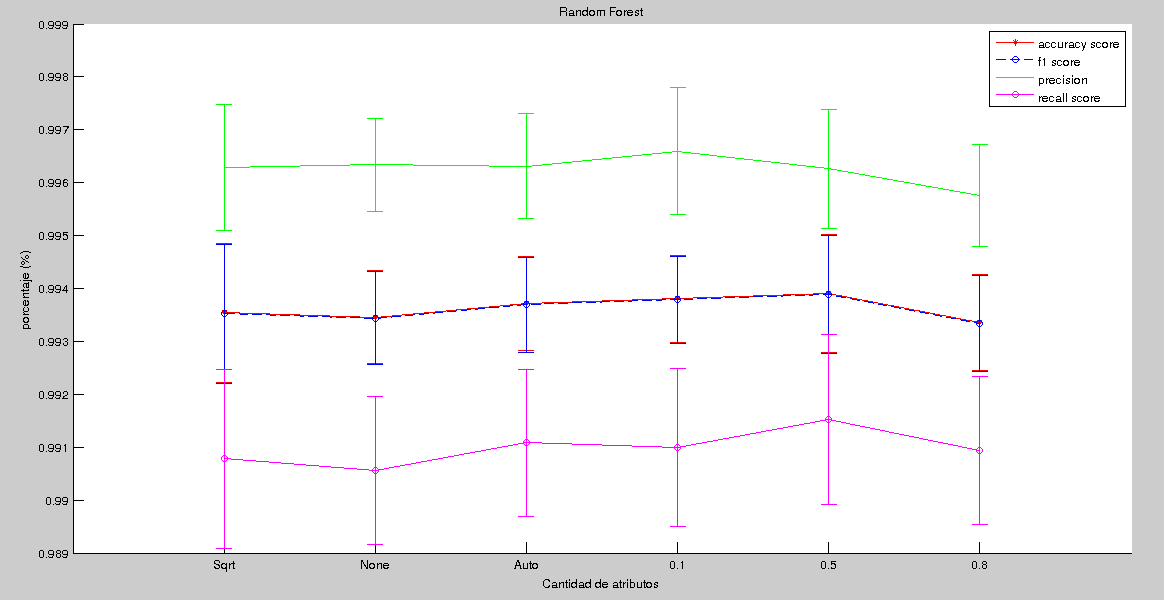
\includegraphics[width=500pt]{randomForestScoresAtributos.png}
\caption{Random Forest con la cantidad de atibutos a considerar variable, 10 arboles y cantidad de features $=$ $\sqrt{cantidad\ original\ de\ features}$}
\label{randomForestAtributos}
\end{center}
\end{figure}

\begin{figure}[H] %[h] Aqui [b] para button [t] para top
\begin{center}
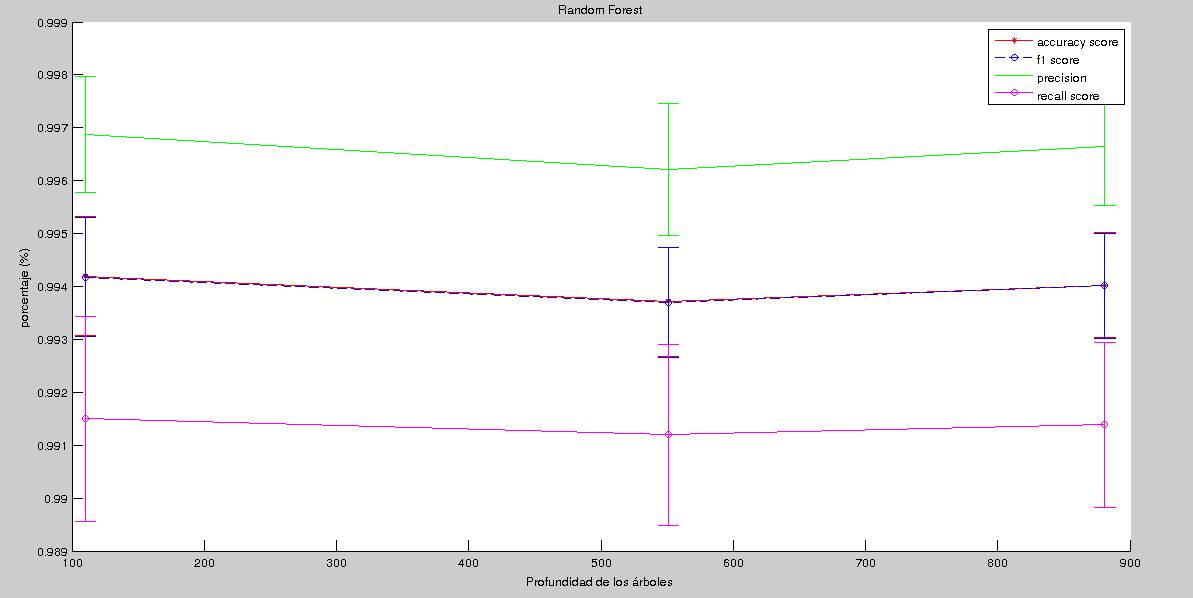
\includegraphics[width=500pt]{randomForestScoreProfundidad.png}
\caption{Random Forest con la profundidad de los árboles variable, 10 árboles y cantidad de features $=$ $\sqrt{cantidad\ original\ de\ features}$}
\label{randomForestProfundidad}
\end{center}
\end{figure}

A partir de las figuras \ref{randomForestArboles}, \ref{randomForestAtributos} y \ref{randomForestProfundidad} pueden estudiarse que combinación de hiperparámetros mejora la predicción sobre los datos experimentales. Puede apreciarse fácilmente que a partir de los 15 árboles considerados, el sistema comienza a complejizarse, y probablemente a sobreajustar los datos, sin proveer mejoras significativas a su capacidad de predicción. Por otro lado, viendo que hay poca diferencia según la cantidad de atributos que se consideran, se decidió tomar la menor cantidad estudiada ya que era la más veloz en entrenarse. En estos casos, el tiempo de entrenamiento variaba entre 2 y 10 segundos según la cantidad de árboles que se utilizaran.

Por último, se decidió entrenar un clasificador cuya combinación de hiperparámetros sea la combinación de los mejores obtenidos. Es decir, se utilizaron 15 árboles y una profundidad y cantidad de atributos (0.1\% de los parámetros totales) a considerar de 110. Este tardo alrededor de 4 segundos en entrenarse y los resultados de su evaluación se presentan en la tabla a continuación.

\begin{center}
  \begin{tabular}{| l | c | c |}
    \hline
      & Porcentaje (\%) & Desvio estandar  \\ \hline
    Accuracy & 0.99455555 & 0.00114665899573 \\ \hline
    F1 & 0.99454728 & 0.00114808481725 \\ \hline
    Precision & 0.99607279 & 0.00145135957533 \\ \hline
    Recall & 0.99302777 & 0.00137465917234 \\
    \hline
  \end{tabular}
\end{center}

\section{Reducción de dimensionalidad}

Una vez evaluados los distintos clasificadores, se seleccionaron como mejores el \textit{Decision Tree} con 110 atributos de profundidad y el \textit{Random Forest} con 15 árboles y 110 atributos de profundidad y considerados en cada división. Se utilizaron dos algoritmos de reducción de dimensionalidad, \textit{Principal Component Analysis} (\textbf{PCA}) o \textit{Latent Semantic Analysis} (\textbf{LSA}), y para evaluar la mejora introducida, se reentrenaron los clasificadores mencionados y se obtuvieron sus parámetros para comparar.

\subsection{Principal component analysis (PCA)}

\textit{Principal Component Analysis} consiste en reducir la dimensión del espacio de atributos utilizando descomposición en valores singulares (\textbf{SVD}) y luego quedándose con los vectores que brindan más información. En este caso, el hiperparámetro a estudiar es la cantidad de parámetros ($\alpha$) que quedarán luego del análisis.

%\todo{En estos gráficos lo haría respecto a la cantidad de vectores q nos quedamos, no respecto a alpha. En los graficos y pasos anteriores siempre mencionamos la cantidad de atributos, no la proporcion. Es por consistencia}

%\todo{Además yo cuento 7 puntos en el results out y aca...}

\begin{figure}[H] %[h] Aqui [b] para button [t] para top
\begin{center}
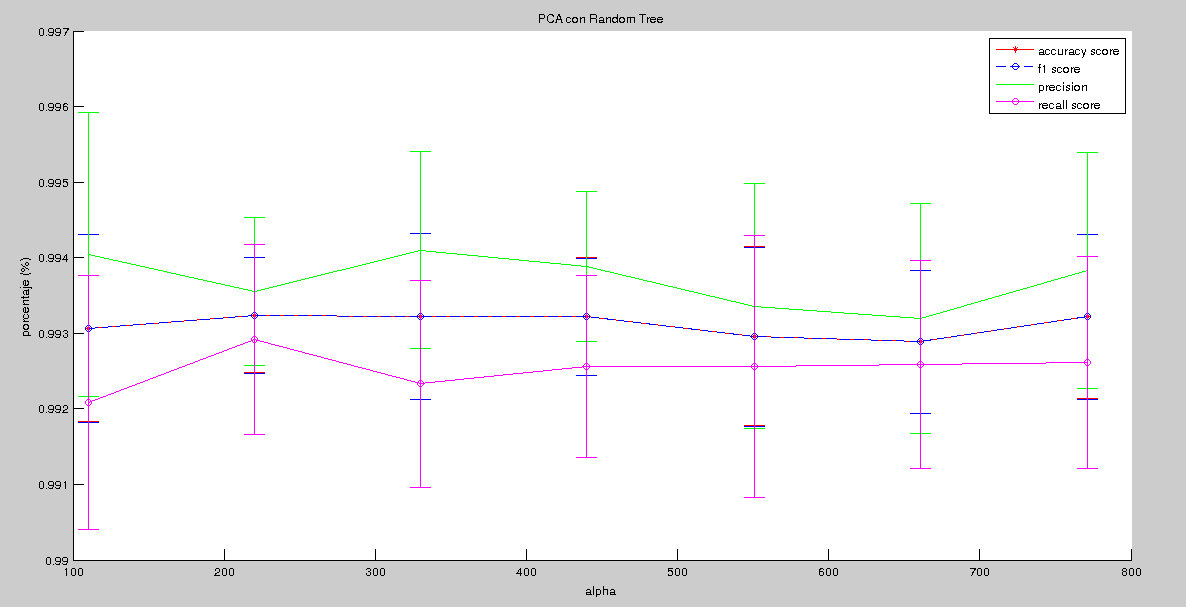
\includegraphics[width=500pt]{pcaRandomTree.png}
\caption{PCA con Random Forest con la cantidad de componentes alpha variable. Se utilizó el clasificador de random forest con 15 árboles, 110 atributos de profundidad y a considerar en cada división.}
\label{pcaRandomTree}
\end{center}
\end{figure}

\begin{figure}[H] %[h] Aqui [b] para button [t] para top
\begin{center}
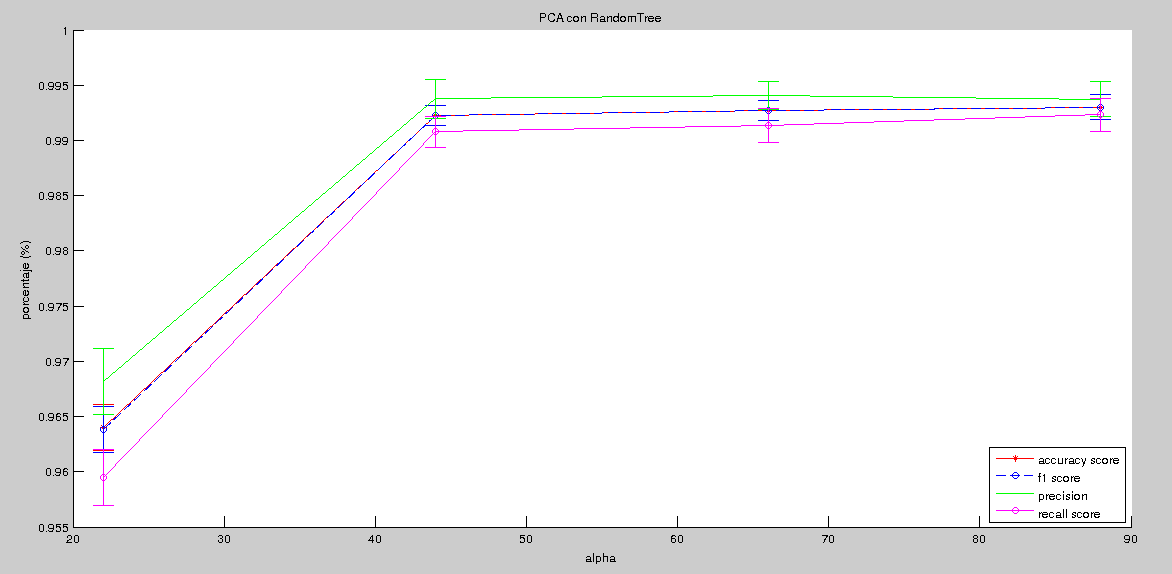
\includegraphics[width=500pt]{pcaRandomTreeZoom.png}
\caption{PCA con Random Forest con la cantidad de componentes alpha variable. Se utilizó el clasificador de random forest con 15 árboles, 110 atributos de profundidad y a considerar en cada división.}
\label{pcaRandomTreeZoom}
\end{center}
\end{figure}

\begin{figure}[H] %[h] Aqui [b] para button [t] para top
\begin{center}
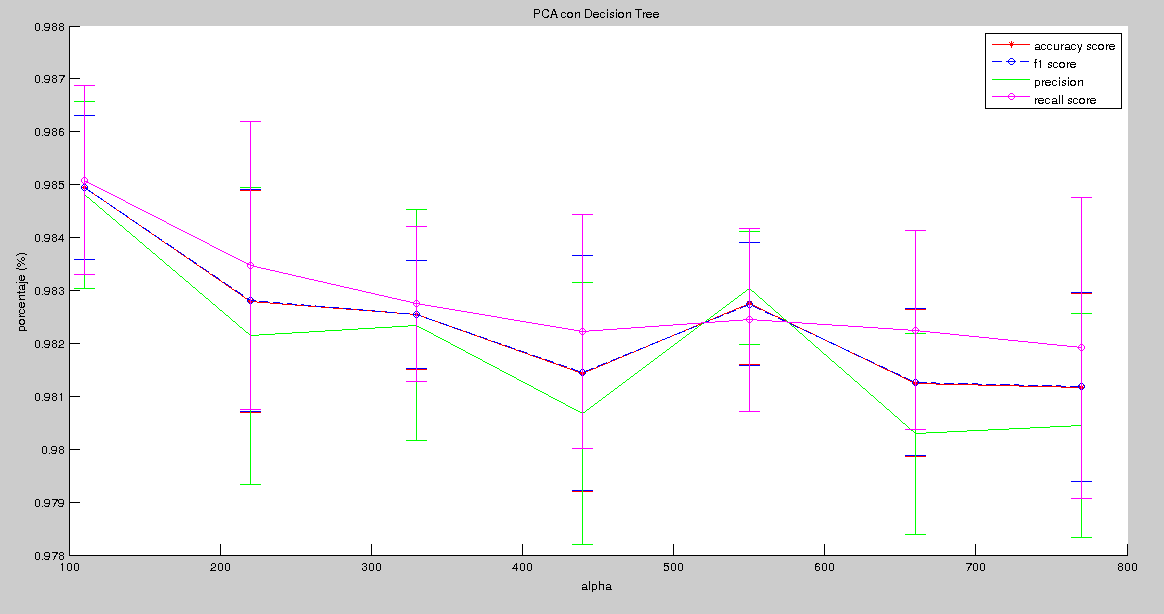
\includegraphics[width=500pt]{pcaDecisionTree.png}
\caption{PCA con Decision Tree con la cantidad de componentes alpha variable. Se utilizó el clasificador de Decision Tree con 110 atributos de profundidad.}
\label{pcaDecisionTree}
\end{center}
\end{figure}

\begin{figure}[H] %[h] Aqui [b] para button [t] para top
\begin{center}
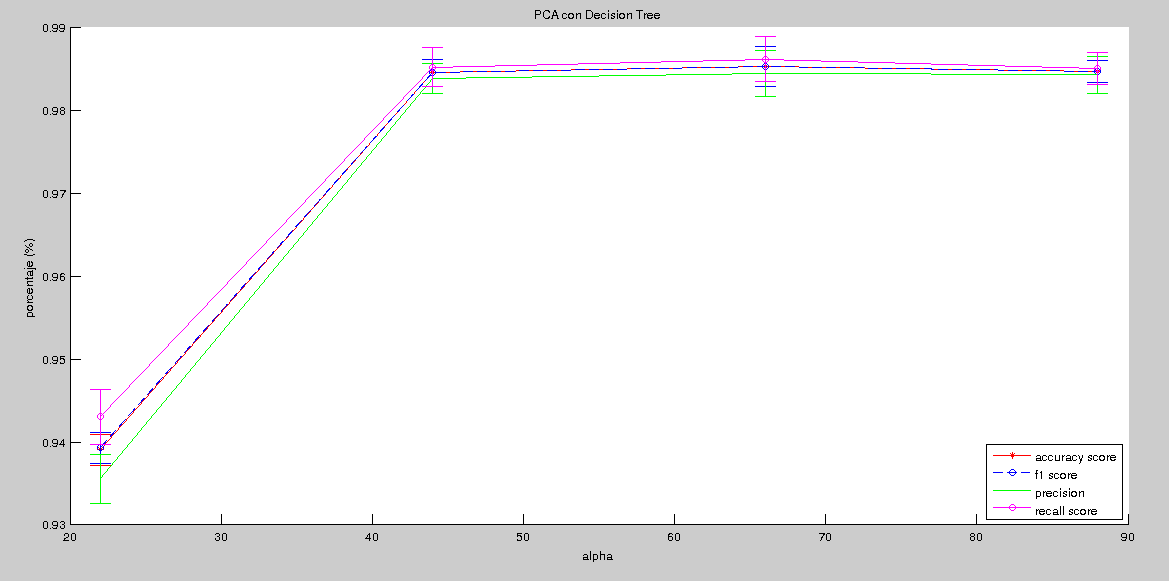
\includegraphics[width=500pt]{pcaDecisionTreeZoom.png}
\caption{PCA con Decision Tree con la cantidad de componentes alpha variable. Se utilizó el clasificador de Decision Tree con 110 atributos de profundidad.}
\label{pcaDecisionTreeZoom}
\end{center}
\end{figure}

Como se puede apreciar en las figuras \ref{pcaRandomTree} y \ref{pcaDecisionTree}, nuestrós parámetros óptimos se encuentran en $\alpha$ = 110. Como éste valor es el borde de nuestro experimento, decidimos generar 2 más tomando valores más chicos ( Figura \ref{pcaRandomTreeZoom} y Figura \ref{pcaDecisionTreeZoom}).

En las figuras \ref{pcaRandomTreeZoom} y \ref{pcaDecisionTreeZoom} puede apreciarse que ambos casos se estabilizan a partir de los 44 vectores. Esto quiere decir que alcanza con tomar esta reducción para apreciar una mejora en el sistema. Aunque el tiempo de entrenamiento en este caso fue del orden del minuto, resulta interesante estudiar que mejoras introduce \textbf{PCA} en el tiempo de predicción para las distintas instancias.

\subsection{Latent Semantic Analysis (LSA)}
\textit{Latent Semantic Analysis} es una técnica que permite comparar las similitudes entre distintos grupos de información. Esta comparación se realiza en un espacio multidimensional generado a partir de la descomposición en valores singulares (\textbf{SVD}). El hiperparámetro que vamos a explorar ($\alpha$) es la cantidad de vectores principales necesarios para tratar de conseguir la mayor información posible.

\begin{figure}[H] %[h] Aqui [b] para button [t] para top
\begin{center}
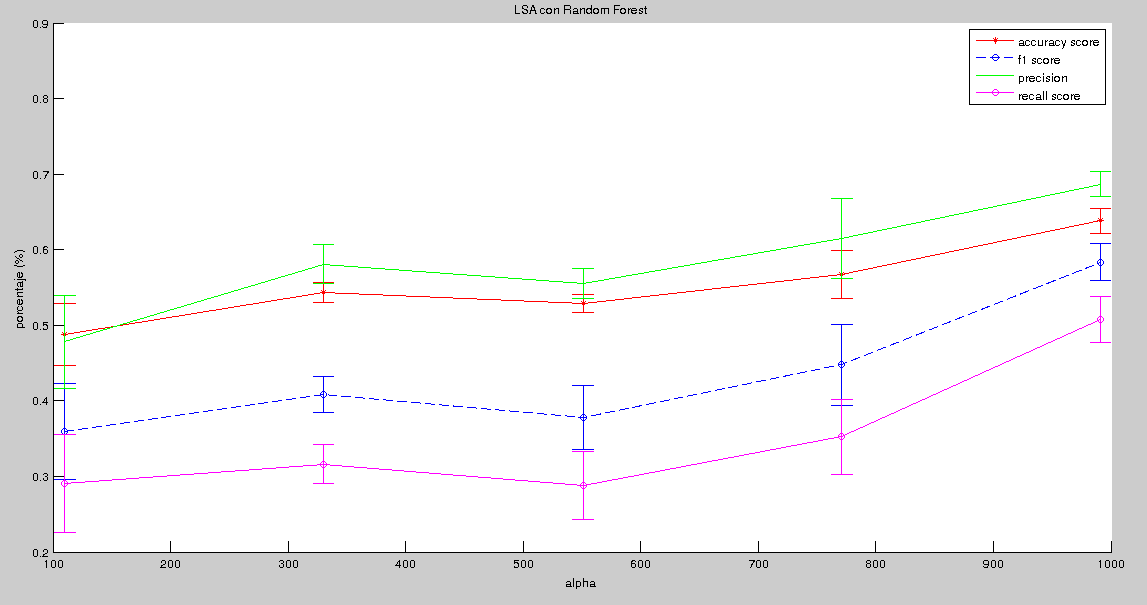
\includegraphics[width=500pt]{lsaRandomForest.png}
\caption{LSA con Random Forest con la cantidad de componentes alpha variable. Se utilizó el clasificador de random forest con 15 árboles, 110 atributos de profundidad y a considerar en cada división.}
\label{lsaRandomTree}
\end{center}
\end{figure}

\begin{figure}[H] %[h] Aqui [b] para button [t] para top
\begin{center}
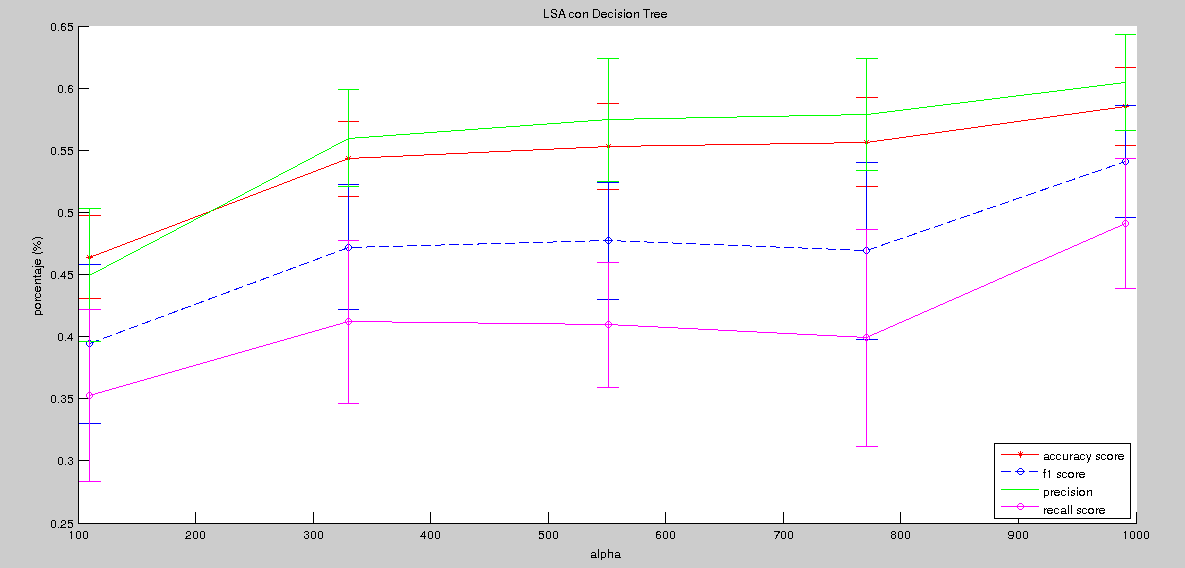
\includegraphics[width=500pt]{lsaDecisionTree.png}
\caption{LSA con Decision Tree con la cantidad de componentes alpha variable. Se utilizó el clasificador de Decision Tree con 110 atributos de profundidad.}
\label{lsaDecisionTree}
\end{center}
\end{figure}

Como se puede observar en las figuras \ref{lsaRandomTree} y \ref{lsaDecisionTree}, los mejores resultados se obtienen al quedarnos con las primeras 990 componentes. El problema de esto, es que al hacerlo, no solo no se obtienen mejores resultados que al aplicar directamente el clasificador sino que tampoco reduce mucho la dimensión del problema original. Es por esta razón que decidimos no tener en cuenta está reducción a la hora de elegir nuestros mejores algoritmos.

\section{Discusión}

\begin{figure}[H] %[h] Aqui [b] para button [t] para top
\begin{center}
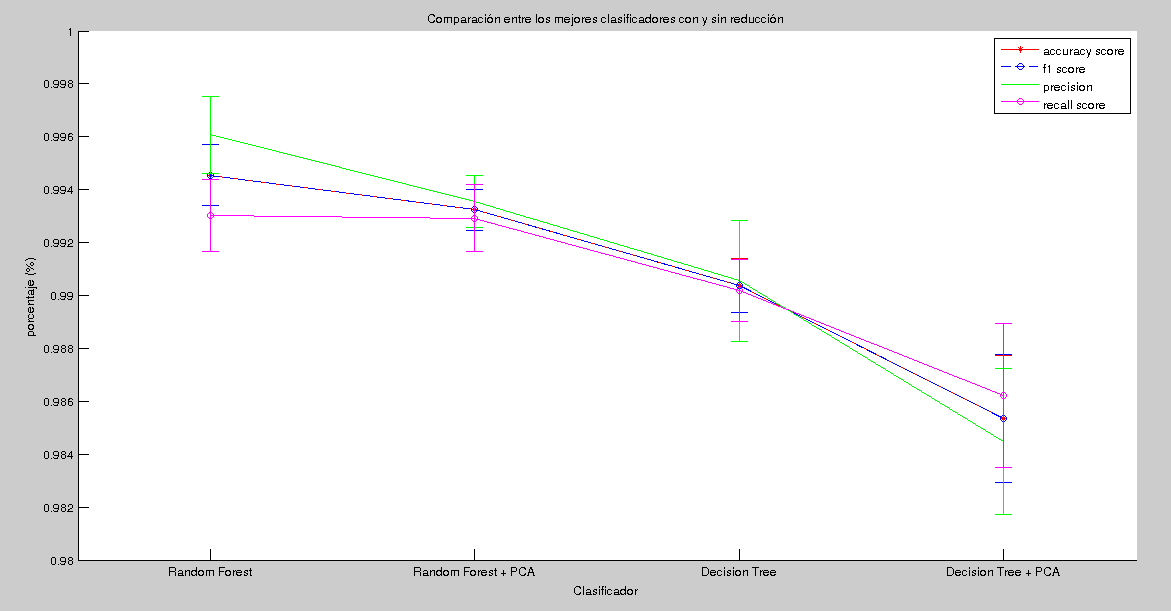
\includegraphics[width=500pt]{compararMetodos.png}
\caption{Comparación entre los 4 métodos con mejores resultados}
\label{compararMetodos}
\end{center}
\end{figure}

Como pudo apreciarse en la sección de Clasificadores, los mejores resultados fueron provistos por \textit{Random Trees} y por \textit{Decision Tree}. Siendo los resultados de \textit{Random Trees} levemente superiores en predicción, aunque 4 veces más lento para entrenar. Por mas que la velocidad de entrenamiento es un parámetro a tener en cuenta, la velocidad de predicción es mucho más importante ya que el entrenamiento se corre una única vez. Se aprecio que la velocidad de procesamiento aumentaba en un orden de magnitud (de 0,4 a 4 segundos al utilizar \textbf{PCA} como método de reducción de dimensionalidad.

Por otro lado, los resultados producidos por \textit{Naive Bayes} eran estadísticamente menores, además que su tiempo de entrenamiento era considerablemente mayor. El caso de K vecinos más cercanos con K=1 (mejor hiperparámetro hallado) tenía una capacidad predictiva aún menor, seguida de un tiempo de entrenamiento cercano al doble de \textit{Naive Bayes}. Es interesante recalcar que los peores resultados fueron obtenidos al utilizar \textit{support vector machines}, donde no solo la capacidad predictiva era considerable y estadísticamente menor a todas, sino que sus tiempos de entrenamiento estaban ordenes de magnitud más altos.

A continuación, se evaluó que sucedía al utilizar \textit{Principal Component Analysis} para reducir la dimensionalidad del espacio de atributos. Es importante recalcar que en este caso se obtuvo una capacidad predictiva comparable a no haber reducido la dimensionalidad. Sin embargo, debe destacarse que, aunque los tiempos de entrenamiento sean mayores, los tiempos de predicción pueden ser menores y la posibilidad de sobreajuste también puede verse reducida considerablemente.

En conclusión, si tenemos el cuenta tanto el tiempo de ejecución como el resultado de la predicción, se puede apreciar que la reducción de dimensionalidad provista por \textbf{PCA} combinada con el clasificador \textbf{RF} provee los mejores resultados sobre el conjunto de datos reservados para evaluar. Dicho esto, nuestro mejor predictor es Random Forest (con 15 árboles, 110 atributos de profundidad y a considerar en cada división) con PCA (con 44 vectores).

A continuación, se evaluaron por separado los métodos de \textbf{RF} con y sin reducción en los datos correspondientes al 10$\%$ guardado para evaluación. Se presentan a continuación los datos obtenidos.

\begin{center}
  \begin{tabular}{| l | c | c |}
    \hline
      & Con Reducción & Sin Reducción  \\ \hline
    Accuracy & 0.9997778 & 0.9997778 \\ \hline
    F1 & 0.9997778 & 0.9997778 \\ \hline
    Precision & 0.9997778 & 0.9997778 \\ \hline
    Recall & 0.9997778 & 0.9997778 \\
    \hline
  \end{tabular}
\end{center}

Habiendo visto que las eficiencias de los distintos métodos son iguales, podemos concluir que utilizar \textbf{RF} con los hiperparámetros elegidos es la mejor opción ya que su tiempo de prediccón es un orden de magnitud más bajo.

Una vez seleccionado el mejor método a implementarse, se evaluó su comportamiento con el último conjunto de datos reservado para evaluación, obteniéndose buenos resultados como se presentan en la tabla a continuación.

\begin{center}
  \begin{tabular}{| l | c |}
    \hline
      & Resultado  \\ \hline
    Accuracy & 0.9883333 \\ \hline
    F1 & 0.9882799 \\ \hline
    Precision & 0.9928235 \\ \hline
    Recall & 0.9837778 \\
    \hline
  \end{tabular}
\end{center}

\end{document}
